\section{Multi-layer networks with non-linearity}
\begin{frame}{Multiple layers}
	\begin{block}{Layers (composition) of $ax+b$ style functions}
		
\includegraphics[width=.5\textwidth, center]{figuras/two_layer_simple.png}
		\begin{align*}
		y &= \mathbb{W} x + b  \\
		z &= \mathbb{U} y + c =\mathbb{U}(\mathbb{W}x+b)+c \\
		  &= (\mathbb{U}\mathbb{W})x + (\mathbb{U}b+c) = \mathbb{V}x+d 
		\end{align*}
	\end{block}
	\begin{block}{Introducing non-linearity with element-wise sigmoid}
		\begin{align*}
		y &= \sigma(\mathbb{W} x + b) \\ 
		z &= \sigma(\mathbb{U} y + c) 
		\end{align*}
	\end{block}
\end{frame}

\begin{frame}{What can these functions (neural networks) do?}
\begin{quote}
	{\small
		A standard multilayer feed-forward network with a locally bounded 
		piecewise continuous activation function can approximate any continuous 
		function to any degree of accuracy if and only if the network's activation 
		function is not a polynomial.\\
		-Leshno et al.,1993
	}
\end{quote}
\begin{quote}
	{\small 
		In particular, we show that arbitrary decision regions can
		be arbitrarily well approximated by continuous feed forward neural networks with
		only a single internal, hidden layer and any continuous sigmoidal nonlinearity.\\
		-Cybenko, 1989 
	}
\end{quote}
\end{frame}

\begin{frame}{Multi-layer, feed forward, non-polynomial}
		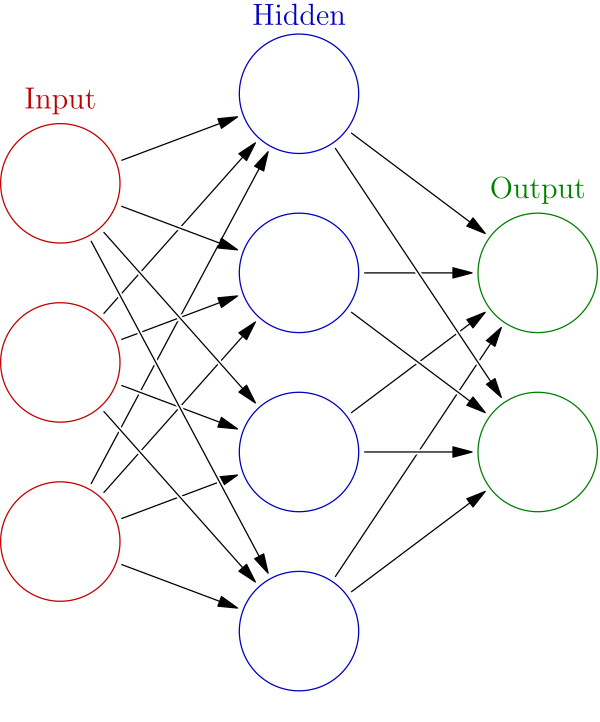
\includegraphics[width=.4\textwidth, center]{figuras/Colored_neural_network_1_hidden.png}
		\tiny{Image from https://en.wikipedia.org/wiki/Artificial\_neural\_network }	
\end{frame}

\begin{frame}{Activation functions}
	\begin{columns}[T]
		\begin{column}{.5\textwidth}
			\tiny{
				\[
				f(x)=\frac{1}{1+e^{-x}}
				\]
			}
			\begin{figure}
				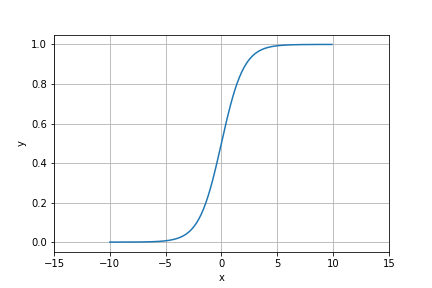
\includegraphics[width=.6\textwidth, center]{figuras/sigmoid.png}	
			\end{figure}
			\tiny{
				\[
				f(x)=\frac{e^x-e^{-x}}{e^x+e^{-x}}
				\]
			}
			\begin{figure}
				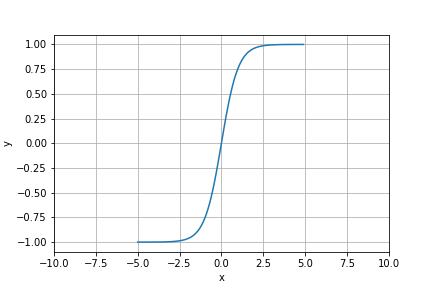
\includegraphics[width=.6\textwidth, center]{figuras/tanh.png}
			\end{figure}
		\end{column}
	%%
		\begin{column}{.5\textwidth}
			\tiny{
				\[
				f(x)=max(x,0)
				\]}
			\begin{figure}
				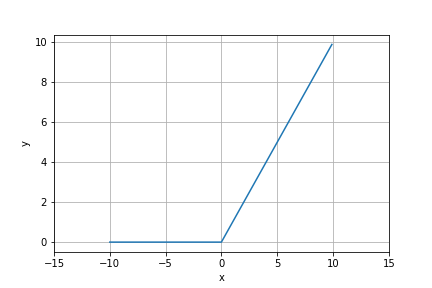
\includegraphics[width=.6\textwidth, center]{figuras/relu.png}	
			\end{figure}
			\tiny{
				\[
				f(x)= 
				\begin{cases}
					x,& \text{if } x\geq 0\\
					0.1x,              & \text{otherwise}
				\end{cases}
				\]
			}
			\begin{figure}
				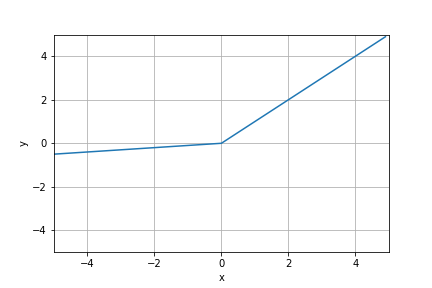
\includegraphics[width=.6\textwidth, center]{figuras/leaky_relu.png}	
			\end{figure}
		\end{column}
	\end{columns}
\end{frame}
